\documentclass[table]{beamer}   

\usepackage{xeCJK}

%\usepackage{indentfirst} 
%\usepackage{hyperref}
%\usepackage{natbib}
%\usepackage{titlesec}
%\usepackage{titletoc}
\usepackage{setspace}%行间距
\usepackage{enumitem} 
\usepackage{booktabs}
\usepackage[justification=centering]{caption}
\usepackage{float}
\usepackage{color}
\usepackage{amsfonts}
\usepackage{array}
\usepackage{tikz}
\usepackage{pgfplots}
\usetikzlibrary{positioning}
\usepackage{amsmath}
\usepackage{setspace}

\usepackage{beamerthemesplit}
\usepackage{subfigure}

\hypersetup{pdfpagemode={FullScreen}}
\usetheme{Madrid}

\renewcommand{\figurename}{图}


\newcommand{\chuhao}{\fontsize{42pt}{\baselineskip}\selectfont}     %初号
\newcommand{\xiaochuhao}{\fontsize{36pt}{\baselineskip}\selectfont} %小初号
\newcommand{\yihao}{\fontsize{28pt}{\baselineskip}\selectfont}      %一号
\newcommand{\erhao}{\fontsize{21pt}{\baselineskip}\selectfont}      %二号
\newcommand{\xiaoerhao}{\fontsize{18pt}{\baselineskip}\selectfont}  %小二号
\newcommand{\sanhao}{\fontsize{15.75pt}{\baselineskip}\selectfont}  %三号
\newcommand{\sihao}{\fontsize{14pt}{\baselineskip}\selectfont}%     四号
\newcommand{\xiaosihao}{\fontsize{12pt}{\baselineskip}\selectfont}  %小四号
\newcommand{\wuhao}{\fontsize{10.5pt}{\baselineskip}\selectfont}    %五号
\newcommand{\xiaowuhao}{\fontsize{9pt}{\baselineskip}\selectfont}   %小五号
\newcommand{\liuhao}{\fontsize{7.875pt}{\baselineskip}\selectfont}  %六号
\newcommand{\qihao}{\fontsize{5.25pt}{\baselineskip}\selectfont}    %七号


\title{基于级联卷积和递归神经网络的蛋白质二级结构预测}
\author{电子与信息工程学院\qquad 计算机科学与技术\\
118532014013\qquad 袁\ 超\qquad 指导教师:游文杰}
\date{}

\begin{document}

\frame{\titlepage}

\begin{frame}{总览}
	\tableofcontents
\end{frame}


\section{蛋白质预测}
\begin{frame}{蛋白质预测}{什么是蛋白质的二级结构?}
\begin{figure}[htbp]
\includegraphics[width=1\textwidth]{pic/ppt105M}
%\caption{
%数据来自RCSB(\url{https://www.rcsb.org/})的蛋白质PDB\ 105M:a)为该蛋白质氨基酸序列,字母代表不同种类的氨基酸残基;b)为该蛋白质的3类二级结构图,颜色代表的类别与(a)中的色彩相对应;c)代表其三级结构的彩虹带图;d)为两条105M蛋白质相互结合形成的四级结构表面图。}
\caption{数据来自RCSB(\url{https://www.rcsb.org/})的蛋白质PDB\ 105M}
\end{figure}
\end{frame}

\begin{frame}{蛋白质预测}{八类蛋白质二级结构预测的符号化定义:}
给定一条蛋白质输入序列$x=(x^{(1)},x^{(2)},\cdots,x^{(n)})^T$,存在模型$f$,使得
\begin{equation}
	y=f(x)=(y^{(1)},y^{(2)},\cdots,y^{(n)})^T
\end{equation}
如果$y^{(i)}\in \{H,G,I,E,B,T,S,C\}_8$,则称$y$为序列$x$的八类二级结构预测结果,$y^{(i)}$为第$i$个残基所对应的二级结构,共八种类别。
\end{frame}

\section{预备知识}
\begin{frame}{预备知识}{预测评估}
设第$i$条蛋白质序列$x_i$有$n_i$个残基,其中正确预测有$m_i$个残基,则
\begin{equation}
	Q_8=\frac{\sum\limits^{N}_{i=1}m_i}{\sum\limits^{N}_{i=1}n_i}
\end{equation}
第$i$条蛋白质的$Q_8$准确率
\begin{equation}
	q_i = \frac{m_i}{n_i}
\end{equation}
也可以参考准确率
\begin{equation}
	r=\frac{1}{N}\sum\limits^{N}_{i=1}\frac{m_i}{n_i}
\end{equation}
\end{frame}


\begin{frame}{预备知识}{梯度下降}
代价函数:
\begin{equation}
	J_{\theta}=\frac{1}{N}\sum_{j=1}^{N}L(y_j, \hat{f}_{\theta}(x_j))	
\end{equation}
梯度下降:
\begin{equation}
	\theta \gets \theta - \eta \nabla_{\theta} J
\end{equation}
\end{frame}

\begin{frame}{预备知识}{位置特异得分矩阵(PSSM)}
	\begin{figure}
		\centering
		\includegraphics[width=0.7\textwidth]{pic/pptpssm}
	\end{figure}
\end{frame}

\begin{frame}{预备知识}{Fixed-size Ordinally-Forgetting Encoding}
给定一条蛋白质序列$x$及其one-hot编码$x'$,则$x$的FOFE编码矩阵$A_{fofe}=(e^{(1)},e^{(2)},\cdots,e^{(t)})^T$
\begin{equation}
	e^{(t)} = \alpha e^{(t-1)}+x'^{(t)}	
\end{equation}

\begin{table}
\rowcolors{2}{blue!15}{blue!30}
\begin{tabular}{l|l}
\rowcolor{blue!70}PROTEIN SEQUENCE & FOFE\\
$w^{(6)},$ & $0,0,0,0,0,0,1$ \\
$w^{(6)},w^{(4)},$ & $0,0,0,0,1,0,\alpha$ \\
$w^{(6)},w^{(4)},w^{(5)},$ & $0,0,0,0,\alpha,1,{\alpha}^2$ \\
$w^{(6)},w^{(4)},w^{(5)},w^{(0)},$ & $1,0,0,0,{\alpha}^2,\alpha,{\alpha}^3$ \\
$w^{(6)},w^{(4)},w^{(5)},w^{(0)},w^{(5)},$ & $\alpha,0,0,0,{\alpha}^3,1+{\alpha}^2,{\alpha}^4$  \\
$w^{(6)},w^{(4)},w^{(5)},w^{(0)},w^{(5)},w^{(4)}$ & ${\alpha}^2,0,0,0,1+{\alpha}^4,{\alpha}+{\alpha}^3,{\alpha}^5$ \\
\end{tabular}
\end{table}

\end{frame}

\begin{frame}{预备知识}{神经元、多输入感知机}
\begin{figure}
	\centering
	\includegraphics[width=0.6\textwidth]{pic/pptmlp}
\end{figure}
\begin{equation}
	f_{\theta}= \sigma(\sum_{i=1}^{n}w^{(i)}x^{(i)}+b)
\end{equation}
\end{frame}

\begin{frame}{预备知识}{卷机神经网络}
设卷积核$w\in K$,$w$与矩阵$I$进行一次卷积运算,则矩阵$I$第$i$行第$j$列的运算结果为:
\begin{equation}
	I'_{i,j}= (I*w)_{i,j}=\sum_{m}\sum_{n}I_{i+m,j+n}w_{m,n}
\end{equation}
\begin{figure}
	\centering
	\includegraphics[width=0.6\textwidth]{pic/pptcnn}
	];
\end{figure}
\end{frame}

\begin{frame}{预备知识}{循环神经网络}
循环神经网络的子结构是一个动态系统
\begin{equation}
	h^{(t)} = f_{\theta}(h^{(t-1)},x^{(t)})
\end{equation}
若保存所有迭代的输出,循环神经网络模型可以构建出如下的映射关系:
\begin{equation}
	f_{\theta}:\{x^{(1)},x^{(2)},\cdots,x^{(t)}\}\to \{h^{(1)},h^{(2)},\cdots,h^{(t)}\}
\end{equation}
\begin{figure}
	\centering
	\includegraphics[width=0.7\textwidth]{pic/pptrnn}
\end{figure}
\end{frame}

\begin{frame}{预备知识}{Gate Recurrent Unit}
\begin{figure}
	\centering
	\includegraphics[width=0.9\textwidth]{pic/pptgru}
\end{figure}
\end{frame}


\begin{frame}{预备知识}{GRU}
\begin{align}
z^{(t)} &= \sigma(W_z x^{(t)}\oplus  U_z h^{(t-1)}+b_z)\\
r^{(t)} &= \sigma(W_r x^{(t)}\oplus U_r h^{(t-1)}+b_r)\\
h'^{(t)}&= tanh(W_h x^{(t)}\oplus U_h(r^{(t)}\otimes h^{(t-1)})+b_h)\\
h^{(t)} &= z^{(t)}\otimes h^{(t-1)}+(1-z^{(t)})\otimes h'^{(t)}
\end{align}
\end{frame}

\section{深度模型架构}
\begin{frame}{深度模型架构}
\begin{figure}
	\centering
	\includegraphics[width=0.5\textwidth]{pic/pptcrnn}
\end{figure}
\end{frame}

\begin{frame}{深度模型架构}{组合嵌入层}
\begin{figure}
	\centering
	\includegraphics[width=0.8\textwidth]{pic/pptlayer0}
\end{figure}
\begin{equation}
	A = concatenate\{A_{0-1},sigmoid(A_{pssm}),A_{bifofe}\}
\end{equation}
\end{frame}

\begin{frame}{深度模型架构}{多尺度卷积层}
\begin{figure}
	\centering
	\includegraphics[width=0.8\textwidth]{pic/pptlayer1}
\end{figure}
\begin{equation}
	C^{(i)} = ReLU((A*K^{(i)})+b^{(i)})
\end{equation}
\end{frame}

\begin{frame}{深度模型架构}{B-GRUs层}
\begin{figure}
	\centering
	\includegraphics[width=0.8\textwidth]{pic/pptlayer2}
\end{figure}
\begin{equation}
	B = concatenate\{C,B^{(1)},B^{(2)},B^{(3)})\}
\end{equation}
\end{frame}

\begin{frame}{深度模型架构}{预测层}
\begin{figure}
	\centering
	\includegraphics[width=0.8\textwidth]{pic/pptlayer3}
\end{figure}

\end{frame}


\section{实验和总结}
\begin{frame}{实验和总结}{数据集:蛋白质序列的长度分布图:}
\begin{figure}
	\centering
	\includegraphics[width=0.7\textwidth]{pic/data_hist}
	\caption{数据源自PSICES CullPDB(\url{http://dunbrack.fccc.edu/PISCES.php})}
\end{figure}
\end{frame}

\begin{frame}{实验和总结}{开发及测试环境}
具体的,深度学习模型用Keras(\url{https://keras.io/})库实现,该库基于深度学习开源框架TensorFlow(\url{https://www.tensorflow.org/})的高级的API。

整个神经网络都在一台带有32GB内存,NVIDIA GTX 1080 Ti GPU,Intel Core i7-8700k CPU的服务器上训练。同时,使用提前停止来防止模型发生过拟合,训练大约需要半天时间。
\end{frame}

\begin{frame}{实验和总结}{模型训练和验证集损失变化}
\begin{figure}
	\centering
	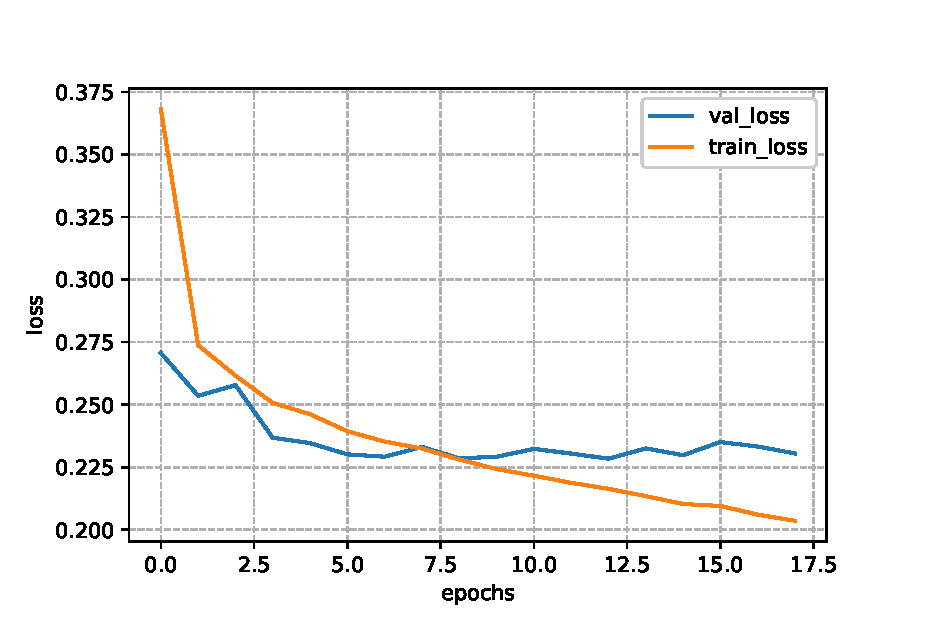
\includegraphics[width=0.7\textwidth]{pic/loss.eps}
	\caption{使用CB6133的99.6\%做训练数据,剩余0.4\%做验证数据}
\end{figure}
\end{frame}


\begin{frame}{实验和总结}{$Q_8$准确率随迭代次数的变化}
\begin{figure}
	\centering
	\includegraphics[width=0.7\textwidth]{pic/val_q8.eps}
	\caption{过滤CB6133的全部数据做训练,用CB513来测试}
\end{figure}
\end{frame}


\begin{frame}{实验和总结}{算法在CB513测试集上的混淆矩阵}
\begin{table}
\scalebox{0.8}{
\begin{tabular}{ccccccccc}
\toprule
 & $H_{pred}$& $B_{pred}$& $E_{pred}$& $G_{pred}$& $I_{pred}$& $T_{pred}$& $S_{pred}$& $L_{pred}$\\
\midrule
$H$& \textbf{92.62}\%& 0.0\%& 0.97\%& 1.1\%&	0.0\%& 2.46\%& 0.3\%& 2.55\%	\\
$B$& 9.14\%& \textbf{1.27}\%& 27.18\%& 0.93\%& 0.0\%& 10.58\%& 5.59\%& 45.3\%\\
$E$& 2.2\%& 0.05\%& \textbf{82.08}\%& 0.46\%& 0.0\%& 2.38\%& 1.53\%& 11.31\%\\
$G$& 27.14\%& 0.0\%& 6.1\%& \textbf{23.63}\%& 0.0\%& 23.21\%& 2.68\%& 17.24\%\\
$I$& 66.67\%& 0.0\%& 3.33\%& 0.0\%& \textbf{0.0}\%& 13.33\%& 3.33\%& 13.33\%\\
$T$& 18.37\%& 0.0\%& 5.38\%& 3.49\%& 0.0\%& \textbf{53.07}\%& 4.49\%& 15.2\%\\
$S$& 8.35\%& 0.02\%& 11.1\%& 1.74\%& 0.0\%& 21.37\%& \textbf{21.38}\%& 36.04\%\\
$L$& 6.17\%& 0.06\%& 17.7\%& 1.03\%& 0.0\%& 8.97\%& 5.48\%& \textbf{60.59}\%\\
\bottomrule
\end{tabular}
}
\end{table}
\end{frame}


\begin{frame}{实验和总结}{算法在CB513测试集上的分类性能比较}	
\begin{table}[htbp]
\center
\begin{tabular}{p{60pt}<{\centering} p{40pt}<{\centering}}
\toprule
算法& $Q_8(\%)$\\
\midrule
CNF& 64.9\%\\
SC-GSN& 66.4\%\\
LSTM large& 67.4\%\\
本文算法& \textbf{68.2}\%\\
\bottomrule
\end{tabular}
\end{table}
\end{frame}

\begin{frame}{演示}
\end{frame}

\begin{frame}{总结}
\centering{\erhao
	Thank you!
	}
\end{frame}

\end{document}
